%% This is file `elsarticle-template-1-num.tex',
%%
%% Copyright 2009 Elsevier Ltd
%%
%% This file is part of the 'Elsarticle Bundle'.
%% ---------------------------------------------
%%
%% It may be distributed under the conditions of the LaTeX Project Public
%% License, either version 1.2 of this license or (at your option) any
%% later version.  The latest version of this license is in
%%    http://www.latex-project.org/lppl.txt
%% and version 1.2 or later is part of all distributions of LaTeX
%% version 1999/12/01 or later.
%%
%% Template article for Elsevier's document class `elsarticle'
%% with numbered style bibliographic references
%%
%% $Id: elsarticle-template-1-num.tex 149 2009-10-08 05:01:15Z rishi $
%% $URL: http://lenova.river-valley.com/svn/elsbst/trunk/elsarticle-template-1-num.tex $
%%
\documentclass[preprint,12pt]{elsarticle}

%% Use the option review to obtain double line spacing
%% \documentclass[preprint,review,12pt]{elsarticle}

%% Use the options 1p,twocolumn; 3p; 3p,twocolumn; 5p; or 5p,twocolumn
%% for a journal layout:
%% \documentclass[final,1p,times]{elsarticle}
%% \documentclass[final,1p,times,twocolumn]{elsarticle}
%% \documentclass[final,3p,times]{elsarticle}
%% \documentclass[final,3p,times,twocolumn]{elsarticle}
%% \documentclass[final,5p,times]{elsarticle}
%% \documentclass[final,5p,times,twocolumn]{elsarticle}

%% The graphicx package provides the includegraphics command.
\usepackage{graphicx}
\usepackage{graphicx}
\usepackage{caption}
\usepackage{subcaption}
%% The amssymb package provides various useful mathematical symbols
\usepackage{amssymb}
%% FOR hyper links
\usepackage{hyperref}
%% The amsthm package provides extended theorem environments
%% \usepackage{amsthm}

%% The lineno packages adds line numbers. Start line numbering with
%% \begin{linenumbers}, end it with \end{linenumbers}. Or switch it on
%% for the whole article with \linenumbers after \end{frontmatter}.
\usepackage{lineno}

%% natbib.sty is loaded by default. However, natbib options can be
%% provided with \biboptions{...} command. Following options are
%% valid:

%%   round  -  round parentheses are used (default)
%%   square -  square brackets are used   [option]
%%   curly  -  curly braces are used      {option}
%%   angle  -  angle brackets are used    <option>
%%   semicolon  -  multiple citations separated by semi-colon
%%   colon  - same as semicolon, an earlier confusion
%%   comma  -  separated by comma
%%   numbers-  selects numerical citations
%%   super  -  numerical citations as superscripts
%%   sort   -  sorts multiple citations according to order in ref. list
%%   sort&compress   -  like sort, but also compresses numerical citations
%%   compress - compresses without sorting
%%
%% \biboptions{comma,round}

% \biboptions{}

\journal{Journal Name}

\begin{document}

\begin{frontmatter}

%% Title, authors and addresses

\title{Unnecessarily Complicated Research Title like : Quantifying information decoded by the brain during artificial proprioceptive feedback. \\ Assessing the performance of a brain-machine interface in stimulation.}

%% use the tnoteref command within \title for footnotes;
%% use the tnotetext command for the associated footnote;
%% use the fnref command within \author or \address for footnotes;
%% use the fntext command for the associated footnote;
%% use the corref command within \author for corresponding author footnotes;
%% use the cortext command for the associated footnote;
%% use the ead command for the email address,
%% and the form \ead[url] for the home page:
%%
%% \title{Title\tnoteref{label1}}
%% \tnotetext[label1]{}
%% \author{Name\corref{cor1}\fnref{label2}}
%% \ead{email address}
%% \ead[url]{home page}
%% \fntext[label2]{}
%% \cortext[cor1]{}
%% \address{Address\fnref{label3}}
%% \fntext[label3]{}


%% use optional labels to link authors explicitly to addresses:
%% \author[label1,label2]{<author name>}
%% \address[label1]{<address>}
%% \address[label2]{<address>}

\author{Julien Rechenmann, Joseph O' Doherty, Philip N. Sabes}

\address{University of California San Francisco (UCSF) \\ Ecole Polytechnique Federale de Lausanne (EPFL)}

\begin{abstract}
%% Text of abstract
LOREM IPSUM POWAAAAAA !
Suspendisse potenti. Suspendisse quis sem elit, et mattis nisl. Phasellus consequat erat eu velit rhoncus non pharetra neque auctor. Phasellus eu lacus quam. Ut ipsum dolor, euismod aliquam congue sed, lobortis et orci. Mauris eget velit id arcu ultricies auctor in eget dolor. Pellentesque suscipit adipiscing sem, imperdiet laoreet dolor elementum ut. Mauris condimentum est sed velit lacinia placerat. Vestibulum ante ipsum primis in faucibus orci luctus et ultrices posuere cubilia Curae; Nullam diam metus, pharetra vitae euismod sed, placerat ultrices eros. Aliquam tincidunt dapibus venenatis. In interdum tellus nec justo accumsan aliquam. Nulla sit amet massa augue.
\end{abstract}

\begin{keyword}
Science \sep Publication \sep Complicated
%% keywords here, in the form: keyword \sep keyword

%% MSC codes here, in the form: \MSC code \sep code
%% or \MSC[2008] code \sep code (2000 is the default)

\end{keyword}

\end{frontmatter}

%%
%% Start line numbering here if you want
%%
\linenumbers

%% main text
\section{Introduction}
\label{S:1}
\subsection{Background and state of the art}

From the National Health Interview Survey (NHIS) of 1996 and the work of \citet{Ziegler-Graham2008}, around 1.6 millions of amputee were estimated living in the United States in 2005. It has been estimated that more than 230'000 people are living with a Spinal Cord Injury (SCI) in the US. These people usually suffer from a partial paralysis of their limb of their body resulting in an incapacity of walking or doing daily motor tasks. Despite rehabilitation, most of them are still unable to move in a natural way. For amputees, mechanic prostheses help to recover a normal activity but are limited in the number of different motor tasks available and their performance compared to natural movement.

Since the control of normal limb is impaired, the idea of controlling machines by "thinking" has been developed. The past few years have seen the rise of brain-machine interfaces (BMI) or brain-computer interfaces (BCI), a new hope for disable people. They allow to control devices like robotic arm or leg prostheses from recorded brain activity. Two categories of BMI have been developed : invasive and non-invasive brain machine interfaces. Both types presents different levels of invasiveness and precision in time and space (figure \ref{fig:bmitypes}). The second one use different kind of devices to record brain activity like functional Magnetic Resonance Imaging (fMRI), Magnetoencephalography (MEG) and Electroencephalography (EEG). They usually offers controls over few choices or classes enabling to use keyboard (\citet{Orhan2012}) or to control a wheelchair (\citet{DelRMillan2009}). Invasive BMI, through Electrocorticography (EcoG) and Utah arrays, allows to have a more control on devices like robotic arm over a 2D plane that can follow a target (\citet{Carmena2003}, \citet{Collinger2013}, \citet{Musallam2004}) or speech recognition (\citet{Brumberg2011}). 

\begin{figure}[htbp]
\centering
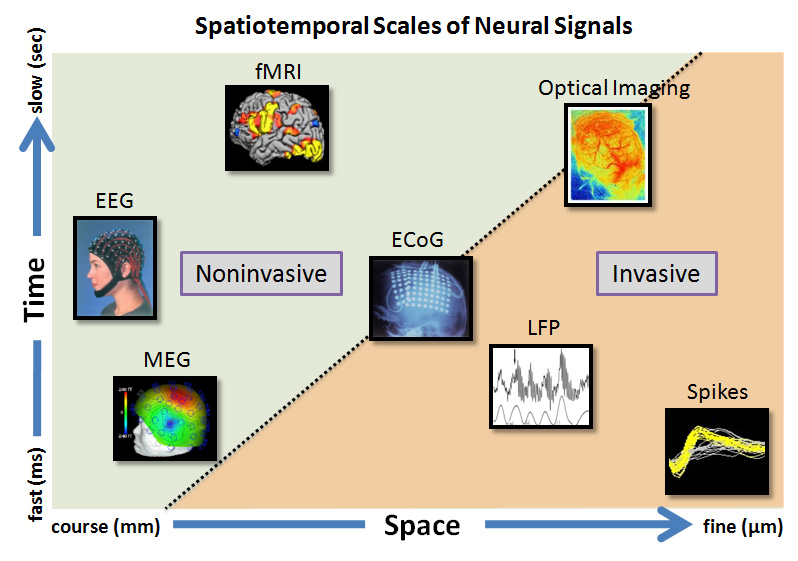
\includegraphics[width=0.75\textwidth]{images/bmitypes.jpg}
\rule{35em}{0.5pt}
\caption[A Utah Array]{\href{http://lifesciences.ieee.org/publications/newsletter/april-2012/96-building-brain-machine-interfaces-neuroprosthetic-control-with-electrocorticographic-signals}{NEEDS TO REMAKE THE FIGURE BY MYSELF (WITHOUT IMAGES TO AVOID PROBLEMS)}}
\label{fig:bmitypes}
\end{figure}

Since the project involves invasive Brain-Machine Interfaces, this section will focus on this type of devices and its performance. Best results have usually been obtained with Utah arrays  and its improved versions since there are known as excellent multi-channel, high-density and long-term neural recordings and stimulation electrodes.
\begin{figure}[htbp]
\centering
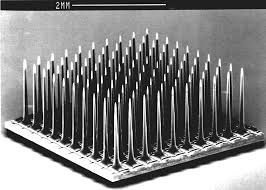
\includegraphics[width=0.75\textwidth]{images/utaharray.jpeg}
\rule{35em}{0.5pt}
\caption[A Utah Array]{\href{http://www.sci.utah.edu/~gk/abstracts/bisti03}{Utah Electrode Arrays developed by the Center for Neural Interfaces.}}
\label{fig:utaharray}
\end{figure}
It has been shown in motor cortex area (M1 see on Figure \ref{fig:monkeybrainarea}),  than neurons are broadly tuned to a specific direction (\citet{Georgopoulos1986}). It means that the frequency of firing of a neuron depends on the direction of the movement and has a preferred direction where the frequency is at its maximum. Through neuronal population direction decoding algorithm, it became possible for implanted monkeys (Utah arrays) to perform simple reaching tasks (\citet{Chapin1999}) and even grasping (\citet{Carmena2003}) tasks. Similar results have been obtained in human (\citet{Hochberg2006}). Neural dynamical models like linear dynamical system (LDS) and Kalman filter have been applied to neuronal recordings from arrays in M1 and dorsal premotor cortex (PMd)  in order to improve the precision of the control of the BMI and facilitate its use (\citet{Kao2015}).
\begin{figure}[htbp]
\centering
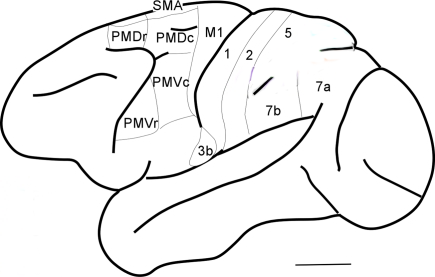
\includegraphics[width=0.75\textwidth]{images/monkeybrain.png}
\rule{35em}{0.5pt}
\caption[A monkey brain scheme]{Macaque brain regions. Utah arrays are usually located in M1 and PMD}
\label{fig:monkeybrainarea}
\end{figure}

These prostheses have been usually implemented in an open-loop process where the feedback of the state of the device is visual. Even though the results obtained through open-loop prosthesis are quite promising, the movement derived from the control is usually not natural and is not as precised as the natural one. During a natural motor task, knowing the state of the limb (proprioception) plays an important role in the feedback and helps to have a more natural movement (\citet{Scheidt2005}). In daily activity, proprioception plays an important role in all motor actions. Research has been led to induce artificial somatosensory feedback through micro-stimulations in S1 region and to compare it to other feedbacks (\citet{Dadarlat2015}, \citet{Godlove2014}).

In order to compare different models of brain activity decoding, multiple tasks have been elaborated and different parameters can be extracted and compared. Reaching Task (\citet{Kao2015}), Tracking Task (\citet{ODoherty2009}) and recently Critical Stability Task (\citet{Quick2014} )seem to be the most revelant. Even though, the most describing parameter is the amount of information in bits per trial or bits per second extracted by the prosthesis from the brain and that allows to perform a task (\citet{Georgopoulos1988}). It leads to many errors during comparison when people have to evaluate the performance of the prosthesis using the same scale but with different tasks. In \citet{Tehovnik2013}, despite the originality of the review, the performance of some prosthesis have been underestimated like for \citet{ODoherty2009} where the performance is estimated to 0.06-0.015 bits/s. Following the method used in the article the real performance is about 0.8 bits/s : there are two different targets (n = 2), the reaching task takes about 1 second (extracted visually from the figures) and the monkey is able to reach correctly 80\% of the targets (even though the aim of the article is to compare the speed of learning and not the performance of the system). As we can see, several attempts has been made to evaluate the performance of the different models elaborated but the results are biased and roughly approximated.



%----------------------------------------------------------------------------------------

\subsection{Aims of the project}
Huge improvements have been made in recent decades using brain-machine interfaces (BMIs) for the control of external devices. However, the quality of control is still erratic, slow and not natural. One hypothesis is that the fluidity of natural movements won't be achieved without somatosensory feedback. Previous work in the lab has shown the possibility of providing artificial feedback about reaching tasks directly into the brain of rhesus monkeys through intra-cortical micro-stimulation (ICMS). The long-term goal of the global project is to create a closed-loop device that will be able to record the intention of movement from the brain and to integrate somatosensory feedback back to the brain using ICMS. The device will be composed of two Utah arrays recording and stimulating in two regions of the brain (M1 and S1, respectively). To assess the degree of improvement that sensory feedback provides the user, it will be necessary to quantify and compare the roles that various types of sensory feedback play in BMI-controlled movements, compare with natural arm movements and identify and model the cortical changes associated with this learning.

My project focused on the evaluation of the impact of degraded feedback on the performance of reaching tasks with different kind of feedback in human (Visual only) and rhesus monkey subjects (Visual, ICMS, visual + ICMS). This step essential to assess the performance of the different methods of decoding and stimulation. The impact of each feedback on reaching skills and the relationship between feedback is also very important to design new experiments. Since the goal was to control a cursor on a screen, a second aim of my project was to define a more natural feedback in a reaching task where the position of the controlled point (2D space) is encoded and not the position of the target. Evaluate its relevance and the performance achieved by the monkey compared to the other models.

Until now, nothing has been done to quantify the amount of information decoded by the brain from artificial proprioceptive feedback. The initial angle bias, parameter extracted from a reaching task, can be related to the amount of information but no approximation of the bits per second extracted from the interface has been done yet. Then, the third goal of my project was to develop a task that allows the quantification of the information the brain extract from a feedback : visual or artificial proprioceptive feedbacks.

\section{Material and methods}
\subsection{Subjects}
For the pilot studies of the new feedback (Magnetic vs Dot Spread), seven human adults between 21 and 28 year old participate to the experiment. No brain disease that could affect motor control have been reported by the subjects. Some of them need to wear glasses during the experiment. For the pilot studies of th Selected Information in Time and Space, only one human subject of 24 year old performed the experiment. The subject (myself) does not have brain disease or eyesight problem during the experiment.

The results for these two experiments have been relevant, so they have been applied on one adult rhesus macaque monkey (Macaca mulatta, 12.5kg). All animal procedures were performed in accordance with the National Research Council’s Guide for the Care and Use of Laboratory Animals and were approved by the UCSF Institutional Animal Care and Use Committee. Training of the monkey and experiments have been lead by me with the help of Joseph O'Doherty. Surgical implantation of the monkey have been done by Prof. Sabes.

Working with monkeys requires several weeks of training and adaptation on daily basis: getting the monkey on the pole, getting it out of the cage to the chair, bringing it to the experiment room, fixing the head, dressing it to prevent any damage to the material, training it to perform the experiment, bringing it back to its cage. This requires to build a relationship of trust between the monkey and the researcher over few weeks or few months.

\subsection{Tasks}
Two different tasks have been used during this project in order to cover most of the movement perform during a daily activity: reaching and stability task. For reaching, we mostly use vision but when it comes to keep an object in the hand (stability), humans and monkeys rely on proprioception to know the state of their body.
\subsubsection{Reaching tasks (RT)}
The reaching task we used consist of moving the arm in order to attain a target uniformly randomly generated on a ring with an inner radius of 40mm and an external radius of 10mm. The monkey has to hold the position of the target for 0.5s. A trial is composed of one or more reach sequences of reaching a random target and coming back to the original position at the center (ADD IMAGE OF A CLASSIC REACHING TASK). This randomly generation is necessary in order to prevent human or monkeys to "learn" how far the target is from the initial position (i.e. when the feedback is degraded).
Reaching tasks have become the simplest and the easiest way to assess the performance of a model applied on a Brain-Machine Interface. The parameters extracted (the reaction time, the reaching duration or the reaching path length) are precised and allow to compare different models. It is also a basic representation of a daily activity for human and monkeys. It is possible to compute the information per trial and the information rate of the decoding through this kind of experiment. In our case, the number of targets is too big to be relevant for computation of information (\ref{eq:inf} and \ref{eq:infrate}). 

\begin{equation} 
Information (Bits) = log_2(N) + Plog_2(P) + (1 - P)log_2(\frac{1-P}{N-1})
\label{eq:inf}
\end{equation}
\begin{equation} 
Infrate (Bits/s) = \frac{Information}{dt}
\label{eq:infrate}
\end{equation}
$N$ is the total number of different targets \\
$P$ is the percentage of targets correctly reached\\
$dt$ is the mean of reaching duration over trials

\subsubsection{Critical Stability Task (CST)}
Critical Stability Task (CST) is a classic task used to evaluate the performance of a system controller (i.e. the ability of a pilot to control an unstable airplane). The goal of the task is to control a unstable system (with transfer function \ref{eq:transfunc} and state function \ref{eq:statefunc}) with the hand or a mouse. The observability of this system is given by $\lambda$ and its controlability is inversely proportional to $\lambda$. Every step T1 (T1 = 1s), the value of lambda increment by 0.1. If the value of the state reached a certain limit(ADD VALUE HERE), the trial stop and we consider the current value of $\lambda$ as the critical lambda $\lambda_c$ where it is not possible anymore to control the systemRecently, it has been used as a main task for psychometric analysis of a feedback (Vibrotactile and visual) in humans and monkeys (\citet{Quick2014}, \citet{Quick2015}).
\begin{equation} 
G = \frac{\lambda}{s-\lambda}
\label{eq:transfunc}
\end{equation}
\begin{equation} 
x(k+1) = e^{\lambda T}x(k) + (e^{\lambda T} - 1)u(k)
\label{eq:statefunc}
\end{equation}
$x(k)$ state of the system at step k\\
$\lambda$ level of instability and observability of the system\\
$T$ time step at which the state of the system is updated (T = 0.03s) \\
$u(k)$ user input (position of the hand or mouse)\\

The main parameters that allows to evaluate the performance of the subject to perform a task is the critical value of $\lambda_c$. In order to use this parameters, we have to consider that the feedback given to the user about the state ($x(k)$) of the system is perfect. Then, change of $\lambda_c$ is correlated to the difficulty of controlling the state of the system.
\subsection{Feedbacks}
For each tasks, multiple feedbacks have been used. Classic normal feedback has been used as control to compare the degraded feedbacks from Dot Spread (DS), Magnetic Target (MT) and Selected Information in Time and Space (SITS). For reaching task, only DS and MT have been used. For CST, MT and SITS have been used. The goal of the DS and MT tasks are to encode the position of the hand or the cursor in order to degrade easily and quantitatively the quality of the feedback. The degradation allows then to compare relatively the quality of the artificial proprioceptive feedback.
\subsubsection{Classic - Visual (C)}
Classis visualization corresponds to the representation on a screen of the position of the hand by a disk of radius 5mm. The target is also represented as a disk of radius 5mm.
\subsubsection{Dot spread - Visual (DS)}
The Dot Spread feedback encodes the position of the hand or the cursor by a certain amount of dots blinking at a frequency of XX Hz in a circle. The number of dots and the size of the circle depends on the degradation (coherence) of the feedback ($ 5 [mm] < r <5/coherence [mm]$). This feedback has only be used on human subject since we wanted to determine which feedback, between DS and MT, had a psychometric curve with the lowest slope in order to find the most learnable feedback for the monkeys.
\subsubsection{Magnetic Target - Visual (MT)}
The Magnetic Target feedback encode the position of the hand or the cursor as a magnetic target. The screen is then covered by numerous lines (compasses) that are attracted by the target. The degradation of the feedback is done by adding random "ghost" targets generated on the screen (not visible) and associated to a certain percentage of compasses: 60\% of compasses get a random ghost target (different for each compass) for 40\% of coherence (figure \ref{fig:feedbacks}). The number of compasses varies between humans and monkeys and between tasks (table \ref{table:lines}). This was needed in order, for the subjects, to learn and perform the task in a non-frustrating way.
\subsubsection{Selected Information in Time and Space - Visual (SITS)}
\subsubsection{Artificial proprioceptiion - Non Visual (AP)}

\begin{figure}[htbp]
\centering
\renewcommand{\thesubfigure}{\Alph{subfigure}}
\begin{subfigure}[b]{0.9\textwidth}
\caption{}
\end{subfigure}
\renewcommand{\thesubfigure}{\Alph{subfigure}}
\begin{subfigure}[b]{0.9\textwidth}
\caption{}
\end{subfigure}
\renewcommand{\thesubfigure}{\Alph{subfigure}}
\begin{subfigure}[b]{1\textwidth}
\caption{}
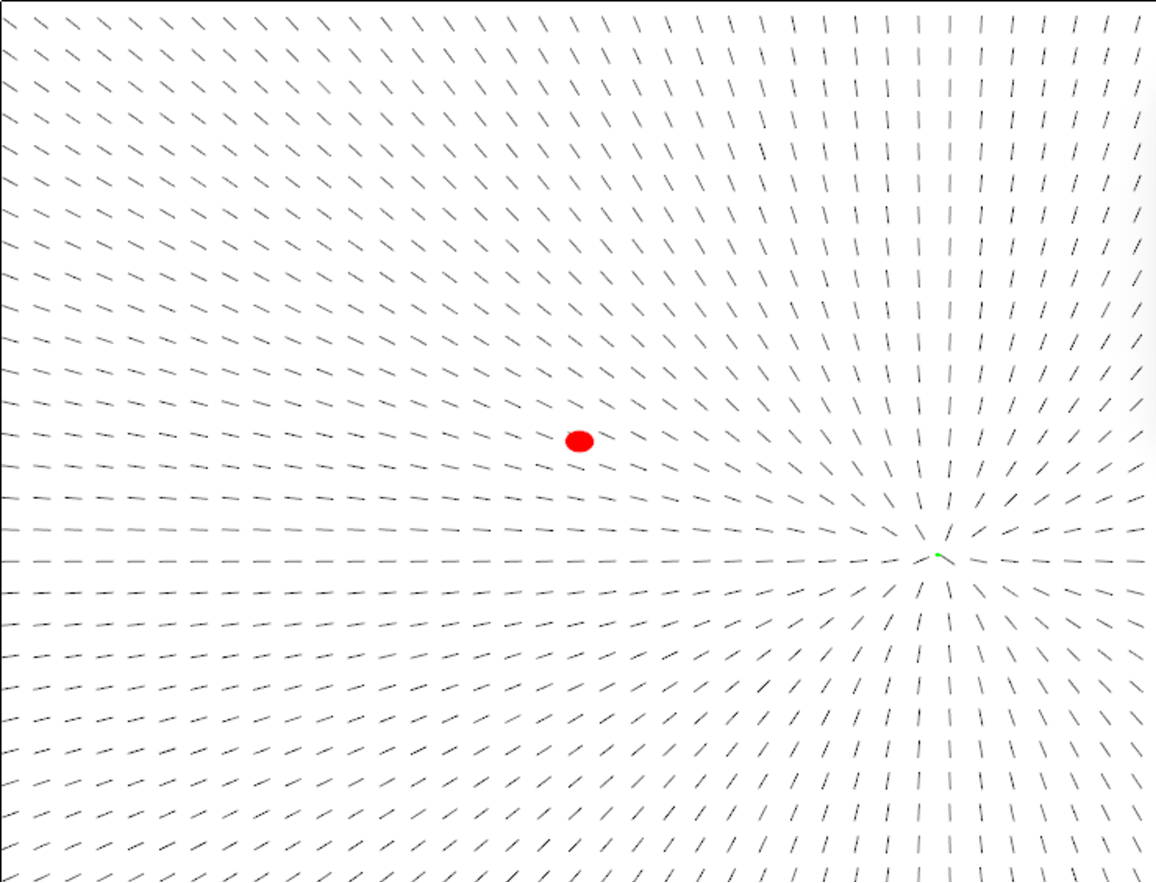
\includegraphics[width=0.49\textwidth,trim={7.5cm 4cm 2.5cm 2.5cm},clip]{images/MTcoherence100.pdf}
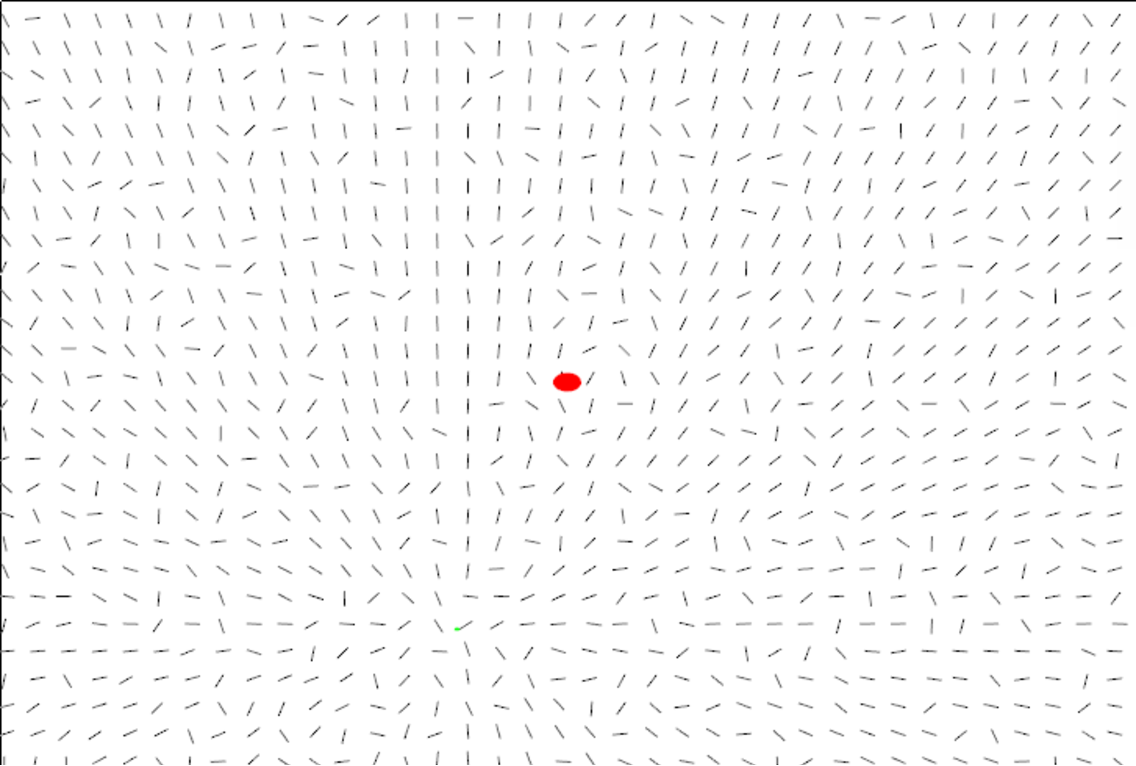
\includegraphics[width=0.49\textwidth,trim={2.5cm 0cm 7.5cm 5cm},clip]{images/MTcoherence50.pdf}
\end{subfigure}
\caption{\textbf{(A)} Classic visual feedback example. \textbf{(B)} Dot Spread feedback example at 100\% (left) and low (right) coherence. \textbf{(C)} Magnetic Target feedback at 100\% (left) and 50\%(right) coherence. The target to reach is drawn in red. The position of the cursor is given by the lines orientation.}
\label{fig:feedbacks}
\end{figure}

\begin{table}
\begin{center}
\begin{tabular}{ |c|c|c|c| } 
 \hline
  & Humans & Monkey I & Monkey L \\ 
 RT & 1000 & 2500 & ???\\ 
 CST & 2000 & ??? & ???\\ 
 \hline
\end{tabular}
\end{center}
\caption{Number of compasses for Reaching and Critical stability task (RT \& CST) depending on human or monkey subject}
\label{table:lines}
\end{table}



\section{Results}
\section{Discussion}
\section{Conclusion}
%% The Appendices part is started with the command \appendix;
%% appendix sections are then done as normal sections
%% \appendix

%% \section{}
%% \label{}

%% References
%%
%% Following citation commands can be used in the body text:
%% Usage of \cite is as follows:
%%   \cite{key}          ==>>  [#]
%%   \cite[chap. 2]{key} ==>>  [#, chap. 2]
%%   \citet{key}         ==>>  Author [#]

%% References with bibTeX database:

\bibliographystyle{model1-num-names}
\bibliography{report}

%% Authors are advised to submit their bibtex database files. They are
%% requested to list a bibtex style file in the manuscript if they do
%% not want to use model1-num-names.bst.

%% References without bibTeX database:

% \begin{thebibliography}{00}

%% \bibitem must have the following form:
%%   \bibitem{key}...
%%

% \bibitem{}

% \end{thebibliography}


\end{document}

%%
%% End of file `elsarticle-template-1-num.tex'.